\documentclass[journal]{IEEEtran}

\usepackage{subfigure}
\usepackage{setspace}
\usepackage[labelsep=period]{caption}  
\usepackage[english]{babel} 
\usepackage{amsfonts,amsmath,bm,bbm}
\usepackage{hyperref} 
\usepackage{graphicx,xurl}
\usepackage{rotating}
\usepackage{todonotes}
\usepackage{lipsum}
\usepackage{xcolor} 
\usepackage{tikz}
\usepackage{ifthen}
\usepackage{color}
\usepackage{multicol,multirow}
\usepackage{float}
\usepackage{siunitx}
\usepackage{algorithm,algorithmicx,algpseudocode}
\usepackage{booktabs}

\renewcommand{\Bbb}{\mathbb}

% Author Orchid ID: enter ID or remove command
%\newcommand{\orcidauthorA}{0000-0001-9647-0506} 
%\newcommand{\orcidauthorB}{0000-0002-8002-5341} 
%\newcommand{\orcidauthorC}{0000-0002-1288-2528} 
%\newcommand{\orcidauthorD}{0000-0003-4523-6466}

\newdimen\HilbertLastX
\newdimen\HilbertLastY
\newcounter{HilbertOrder}

\def\DrawToNext#1#2{%
\advance \HilbertLastX by #1
\advance \HilbertLastY by #2
\pgfpathlineto{\pgfqpoint{\HilbertLastX}{\HilbertLastY}}
}

% \Hilbert[right_x,right_y,left_x,left_x,up_x,up_y,down_x,down_y]
\def\Hilbert[#1,#2,#3,#4,#5,#6,#7,#8] {
\ifnum\value{HilbertOrder} > 0%
\addtocounter{HilbertOrder}{-1}
\Hilbert[#5,#6,#7,#8,#1,#2,#3,#4]
\DrawToNext {#1} {#2}
\Hilbert[#1,#2,#3,#4,#5,#6,#7,#8]
\DrawToNext {#5} {#6}
\Hilbert[#1,#2,#3,#4,#5,#6,#7,#8]
\DrawToNext {#3} {#4}
\Hilbert[#7,#8,#5,#6,#3,#4,#1,#2]
\addtocounter{HilbertOrder}{1}
\fi
}

% \hilbert((x,y),order)
\def\hilbert((#1,#2),#3){%
\advance \HilbertLastX by #1
\advance \HilbertLastY by #2
\pgfpathmoveto{\pgfqpoint{\HilbertLastX}{\HilbertLastY}}
\setcounter{HilbertOrder}{#3}
\Hilbert[1mm,0mm,-1mm,0mm,0mm,1mm,0mm,-1mm]
\pgfusepath{stroke}%
}

% correct bad hyphenation here
\hyphenation{op-tical net-works semi-conduc-tor}


\begin{document}

\title{Analysis and Classification of SAR Textures using Information Theory}

\author{Eduarda~T.~C.~Chagas, %\orcidA{}
	Alejandro~C.~Frery, %\orcidB{}
	\IEEEmembership{IEEE~Senior~Member,}
	Osvaldo~A.~Rosso, %\orcidC{}
	and~Heitor~S.~Ramos %\orcidD{}
	
	\thanks{E.\ T.\ C.\ and H.\ S.\ Ramos ar with Departamento de Ci\^encia da Computa\c c\~ao, Universidade Federal de Minas Gerais, Belo Horizonte, Minas Gerais, Brazil (e-mail: eduarda.chagas@dcc.ufmg.br, ramosh@dcc.ufmg.br).}
	\thanks{A.\ C.\ Frery is with Laborat\'orio de Computa\c c\~ao Cient\'ifica e An\'alise Num\'erica -- LaCCAN, Universidade Federal de Alagoas, Brasil; (e-mail: acfrery@laccan.ufal.br)}
	\thanks{O.\ A.\ Rosso is with Instituto de F\'isica, Universidade Federal de Alagoas, Brasil (e-mail: oarosso@if.ufal.br)}
	\thanks{Manuscript received XX YY, 20ZZ; revised WW UU, 20VV.}}


\markboth{IEEE JOURNAL OF SELECTED TOPICS IN APPLIED EARTH OBSERVATIONS AND REMOTE SENSING}
%\markboth{IEEE JOURNAL OF SELECTED TOPICS IN APPLIED EARTH OBSERVATIONS AND REMOTE SENSING,~Vol.~13, No.~9, September~2014}%
{Shell \MakeLowercase{\textit{et al.}}: Bare Demo of IEEEtran.cls for Journals}

\maketitle

\begin{abstract}
	We propose a new technique texture analysis and classification based on the Bandt-Pompe symbolization, and we apply it to SAR data.
	It consists of
	(i)~linearize a 2-D patch of the image using the Hilbert-Peano curve,
	(ii)~build an Ordinal Pattern Transition Graph that considers the data amplitude encoded into the weight of the edges;
	(iii)~obtain a probability distribution function derived from this graph;
	(iv)~compute Information Theory descriptors (Permutation Entropy and Statistical Complexity) from this distribution, and use them as features to feed a classifier.
	The ordinal pattern graph we propose considers that the weight of the edges is related to the absolute difference of observations, which encodes the information about the data amplitude. 
	This modification takes into account the scattering properties of the target and leads to the characterization of several types of textures.
	Experiments with data from Munich urban areas, Guatemala forest regions, and Cape Canaveral ocean samples show the effectiveness of our technique, which achieves satisfactory levels of separability.
	The two descriptors chosen in this work are easy and quick to calculate and are used as input for a k-nearest neighbor classifier.
	Experiments show that this technique presents results similar to state-of-the-art techniques that employ a much larger number of features and, consequently, require a higher computational cost.
\end{abstract}

\begin{IEEEkeywords}
	Synthetic Aperture Radar (SAR), 
	Time-series, 
	Texture, 
	Classification, 
	Ordinal Patterns Transition Graphs.
\end{IEEEkeywords}

\IEEEpeerreviewmaketitle

\section{Introduction}

\IEEEPARstart{T}{exture} is an elusive trait.
When dealing with remotely sensed images, the texture of different patches carries relevant information that, more often than not, is hard to quantify and to transform into useful and parsimonious features.
This may be due to the fact that texture, in this context, is a synesthesia phenomenon that triggers tactile responses from visual inputs.
This paper presents a new way of extracting features from textures, both natural and resulting from anthropic processes, in SAR (Synthetic Aperture Radar) imagery.

SAR systems are a vital source of data because they provide high-resolution images in almost all weather and day-night conditions.
They provide basilar information, complementary to that offered by sensors that operate in other regions of the electromagnetic spectrum, for a variety of Earth Observation applications.

SAR data are rich in information, although with challenging characteristics.
Most notably, they do not follow the usual Gaussian additive model, and the signal-to-noise ratio is usually low.

Yue et al~\cite{Yue2020Gaussian} provide a comprehensive account of how the physical properties of the target are translated into first- and second-order statistical properties of SAR intensity data.

There is general agreement that non-deterministic textures are encoded in the second-order features, i.e., in the spatial correlation structure.
This notion often leads to using the covariance matrix and other measures that assume that a linear dependence, namely the Pearson correlation coefficient, suffices to characterize natural textures.

For the aforementioned reasons, this might not be the case when dealing with SAR imagery.
Texture, in these images, is often visible only over large areas, and the multiplicative and non-Gaussian nature of speckle antagonizes with the additive assumption that underlies classical approaches.

SAR textures can be studied following two complementary approaches, namely analyzing the marginal properties of the data (first-order statistics), and observing their spatial structure~\cite{Yue2020Gaussian, numbisi2018multi}.
In this work, we focus on the second.

%Surface classification and land use are some of the most valuable applications of SAR images.
%
%, and the development of efficient strategies to cope with this problem is an ongoing research topic~\cite{Pottier2004Unsupervised}, for which supervised and unsupervised classification algorithms have been proposed~\cite{han2020unsupervised,huang2020classification,xie2020polsar}.
%Such methods can be divided into two categories: methods based on SAR image statistical information, and methods based on textural information~\cite{guan2019covariance}.
%%
%Extraction and analysis of characteristics are crucial steps in the classification of regions, along with additional information and previous knowledge about the scene, the sensor, and the acquisition conditions.
%The study of SAR textures reveals useful information about the target under analysis, being extremely important to characterize it quantitatively.

%The tonal values in a synthetic aperture radar (SAR) image represent point measurements of the backscatter coefficient, and are related to the radar wavelength and to the interaction with the elements in the scene.
%Through textural information, we acquire data from the spatial distribution of gray levels of the image and statistics about it~\cite{AGeneralizedGaussianCoherentScattererModelforCorrelatedSARTexture}.

%The study of textures in remote sensing presents peculiarities concerning the analysis of isolated patterns since the texture represents only part of the scene under investigation, and it is necessary to consider micro and macro-textural structures of the image during the characterization.
%However, texture analysis in SAR images provides essential information in addition to image gray levels or backscatter values and demonstrates improvements in accuracy in surface characterization due to the structural properties of different regions.

%Feature extraction followed by classification have often been applied, becoming the two significant steps that formed the basis for the analysis of satellite images~\cite{feng2014amplitude}.
%Different measures of texture proved to be essential for satellite images to derive the spatial contour of the surface, the arrangement and other varieties of soil properties.

The most widely used approach to obtain textural features from SAR imagery is through co-occurrence matrices and Haralick's descriptors~\cite{yu2019detection}.
Radford et al.~\cite{radford2018geological} used textural information derived from gray-level co-occurrence matrices, along with Random Forests, for geological mapping of remote and inaccessible localities; the authors obtained a classification accuracy of $\approx\SI{90}{\percent}$, even when using limited training data ($\approx\SI{0.15}{\percent}$ of the total data). 

Hagensieker and Waske~\cite{hagensieker2018evaluation} evaluated the synergistic contribution of multi-temporal L-, C-, and X-band data to tropical land cover mapping, comparing classification outcomes of ALOS-2~\cite{kankaku2013alos}, RADARSAT-2~\cite{morena2004introduction}, and TerraSAR-X~\cite{breit2009terrasar} 
datasets for a study site in the Brazilian Amazon using a wrapper approach. 
The wrapper utilizes the gray-level co-occurrence matrix (GLCM)
texture information and a  Random Forest classifier to estimate scene importance. 

Storie~\cite{storie2018urban} proposed an open-source workflow for detecting and delineating the urban-rural boundary using Sentinel-1a SAR data.
The author used a combination of GLCM information and a k-means classifier to produce a three-category map that distinguishes urban from rural areas. 
Other approaches include the Fourier power  spectrum~\cite{Florindo2012Fractal}, and random fields~\cite{zhu2016antarctic}.

In our approach, we opt to analyze the 1-D signals resulting from the linearization of the image samples, using non-parametric time series analysis techniques.
With this approach, we reduce the dimensionality of the data and map the spatial dependence of the pixels onto the temporal correlation of a time series.
Next, we extract a probability distribution from the ordinal patterns of a new transition graph, herein proposed, which can discriminate different levels of amplitude, and we use well-known features borrowed from the Information Theory field to classify texture patches.

The main contribution of this work is the proposal of a new set of features for characterization and classification of SAR textures, based on a modification of the current ordinal patterns transition graph, incorporating relevant time-series information.
Our proposal, hereinafter referred to as Weighted Amplitude Transition Graph (WATG), incorporates the absolute difference between the observations, weighting them in the calculation of the final value of their probabilities.
Experiments performed on SAR image textures indicate that this approach preserves essential information about the dynamics of the system, presenting excellent results in the classification of regions, where it has reached satisfactory levels of separability.

The paper is structured as follows:
Section~\ref{methodology} describes our proposed methodology.
Section~\ref{linearization} presents the patch linearization process of the images.
Section~\ref{WATG} shows our technique of ordinal amplitude transition graph weighting by amplitudes.
In Section~\ref{HC} we report the Information Theory descriptors used throughout this work.
Section~\ref{Results} describe the SAR image datasets, 
the analysis of ordinal pattern methods, 
experiments of sliding window selection, 
and a quantitative assessment.
Finally, Section~\ref{Conclusion} concludes the paper.

\section{Methodology}\label{methodology}

The methodology applied in this work is shown in Alg.~\ref{alg:watg}.
The main idea of the technique is as follows.
After receiving the P texture patch, the algorithm linearizes the image using Hilbert-Peano curves, thus acquiring a time series.
Then, the procedure calls the \texttt{WATG} subroutine over the time series and the ordinal pattern parameters to calculate the probability distribution.
Finally, shannon permutation entropy and statistical complexity are calculated.
This features obtained in the last step can be used either for characterization or classification.

The \texttt{WATG} function basically consists of three steps: ~(i) we use the embedding dimension $D$ and time delay $\tau$ in \texttt{BPSymbolization} subroutine for generate the ordinal patterns of the given time series using Bandt-Pompe, ~(ii) with the symbols in hand, the \texttt{transitions} function calculates the sequence of alternations of the ordinal patterns, and in ~(iii) \texttt{weigthGraph} generates the desired incidence matrix of the graph using the weights of the amplitude differences between the time series elements.
Finally, the probability distribution obtained by the proposed method is achieved by vectoring the final transition matrix.
These steps are also depicted in Fig.~\ref{fig:WATG}, and are detailed in the following sections.

\begin{algorithm}[h]
	\caption{$H \times C$ point from a patch using WATG}
	\label{alg:watg}                                
	\textbf{Input:} Patch of texture $P$, dimension $D$ and time delay \textbf{$\tau$}\\
	\textbf{Output:} $H \times C$ feature
	\begin{algorithmic}[1]
		\State time.series $\gets$ \texttt{hilbertCurve}($P$)
		\State Probs $\gets$ \texttt{WATG}(time.series, D, $\tau$)
		\State H $\gets$ \texttt{ShannonEntropy}(Probs)
		\State C $\gets$ \texttt{StatisticalComplexity}(Probs)
		
		\vspace{0.15cm}
		
		\Function{\texttt{WATG}}{time.series, D, $\tau$}
		\State patterns $\gets$ \texttt{BPSymbolization}(time.series, D, $\tau$)
		\State transitions $\gets$ \texttt{transitions}(patterns)
		\State graph $\gets$ \texttt{weigthGraph}(time.series, transitions)
		\State Probs $\gets$ \texttt{as.vector}(graph)
		\State \Return Probs
		\EndFunction
	\end{algorithmic}
\end{algorithm}


\begin{figure}[hbt]
	\centering
	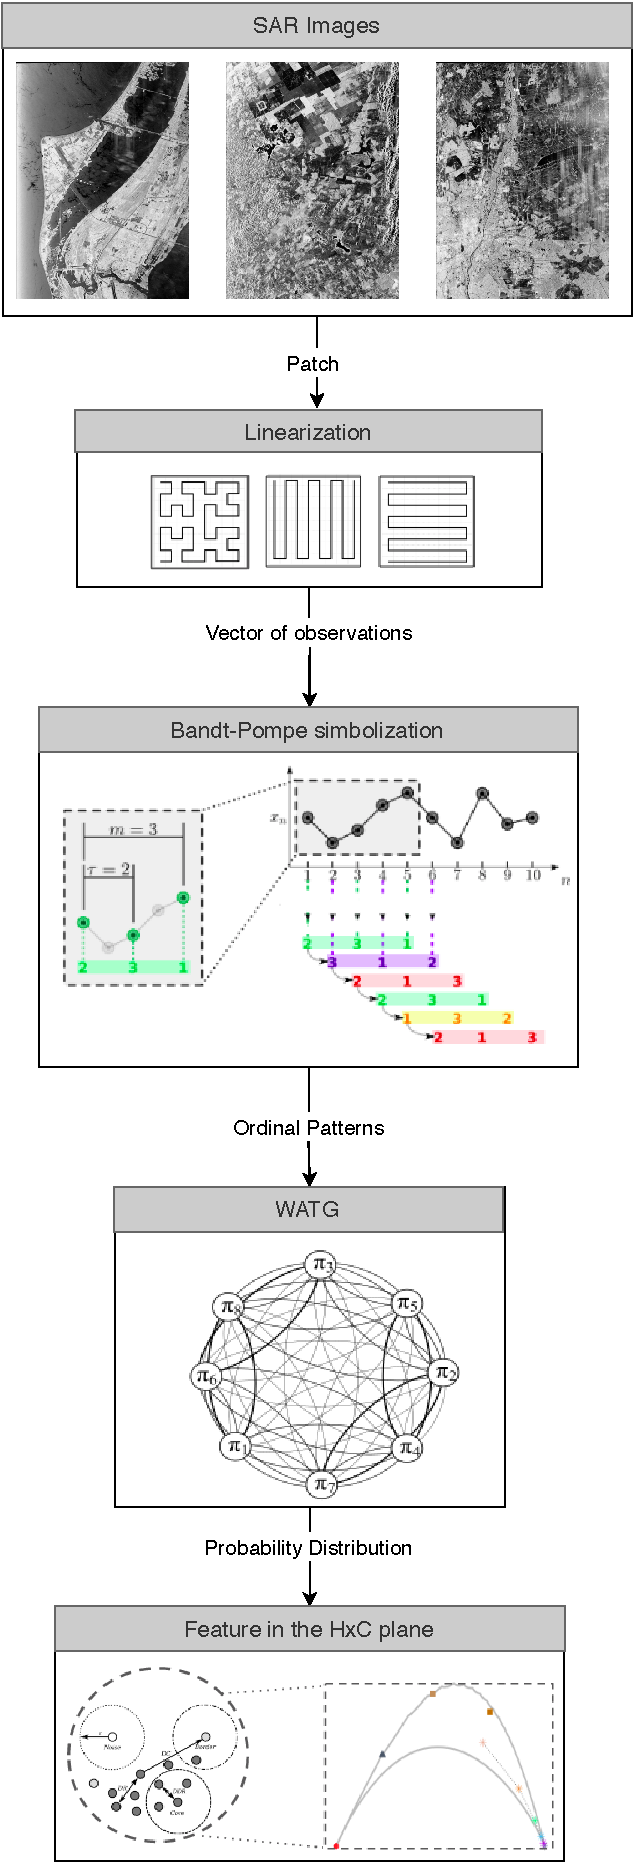
\includegraphics[width=.7\columnwidth]{Figures/methodology.pdf}
	\caption{Outline of the methodology used for the classification of textures.}
	\label{fig:WATG}
\end{figure}

\subsection{Linearization of image patches}\label{linearization}

In this step, we perform a data dimensionality reduction by turning the 2-D patch into a times series, i.e., a 1-D signal.
This could be accomplished by reading the data by lines, columns, or any transformation of 2-D indexes into a sequence of integers.
In this work, we choose to use the Hilbert-Peano curve~\cite{Lee1994Texture}.

Nguyen et al.~\cite{nguyen1982space} firstly employed Space-filling curves, to map texture into a one-dimensional signal.
%\todo[inline]{isso não era para ser uma citação?}
%%% ETCC DONE
When used as scanning methods of an image, such functions preserve relevant properties of pixel spatial correlation~\cite{Lee1994Texture}.

Carincotte et al.~\cite{Carincotte2006changeDetection} used the Hilbert-Peano curve in the problem of change detection in pairs of SAR images.
The authors noted that this transformation exploits the spatial locality and that its pseudo-randomness
of direction changes works well for a large family of images, especially
natural ones.

Assuming an image patch is supported by an $M \times N$ grid, we have the following definition.

\newtheorem{mydef}{Definition}
\begin{mydef}
	An image scan is a bijective function $f \colon \mathbb{N} \times \mathbb{N} \to \mathbb{N}$ in the ordered pair set $ \{(i, j): 1 \leq i \leq M , 1 \leq j \leq N\}$, which denotes the points in the domain, for the closed range of integers $\{1, \dots, M  N\}$.
	A scan rule is $\{f^{-1}(1), \dots, f^{-1}(M  N)\}$.
	\label{def:CurveFilling}
\end{mydef}
This Definition imposes that each pixel is visited only once, and that all pixels are visited.

Space-filling curves, such as raster-1, raster-2, and Hilbert-Peano scanning techniques, stipulate a proper function $f$.
Traditional Hilbert-Peano curves scan an array of pixels of dimension $2^k \times 2^k$, $k \in \mathbb{N}$, never keeping the same direction for more than three consecutive points, as shown in Fig.~\ref{fig:Hilbert}.
Using the Hilbert-Peano curve, we reduce the data dimensionality by maintaining the spatial dependence information of the patch.
In this work, we use patches of size $128 \times 128$.

\begin{figure}[hbt]
	\centering
	\tikz[scale=3.2] \hilbert((0mm,0mm),3);
	\hspace{0.3cm}
	\tikz[scale=1.5] \hilbert((0mm,0mm),4);
	\hspace{0.3cm}
	\tikz[scale=0.73] \hilbert((0mm,0mm),5);	
	\caption{Visual representation of Hilbert-Peano curve in areas of: (a) $8 \times 8$, (b) $16 \times 16$ and (c) $32 \times 32$. }\label{fig:Hilbert}
\end{figure} 

%%% ACF Reescrever depois de colocar os passos em forma de algoritmo
%%% ETCC Reescrito

%%% ACF Acho melhor organizar o fluxo de ideias. Primeiro esgota-se BP, depois fala-se do grafo de transições, e só depois aparecem os pesos. Idealmente, cada parte fará referência a um passo do algoritmo.
%%% ETCC Organizar o fluxo de acordo com as funções usadas no algoritmo

\subsection{Bandt-Pompe Symbolization}\label{BP}

%Step~\ref{item:WOPTG} consists of two stages.
%In the first, the time series is transformed into a sequence of ordinal patterns.
%In the second, we build a weighted graph describing the transitions between these patterns.

The representation of time series by ordinal patterns was introduced by Bandt and Pompe~\cite{Bandt2002Permutation} as a transformation resistant to noise, and invariant to nonlinear monotonic transformations.
Therefore, the first step of the \texttt{WATG} subroutine is to calculate the ordinal patterns of the time series by Band-Pompe symbolization.

Consider ${\mathcal X} \equiv \{x_t\}_{t=1}^{T}$ a real valued time series of length $T$. 

Let ${\mathfrak A}_{D}$ (with $D \geq 2$ and $D \in {\Bbb N}$) be the symmetric group of order $D!$ formed by all 
possible permutation of order $D$, and the symbol component vector 
${\bm \pi}^{(D)} = (\pi_1, \pi_2, \dots, \pi_D)$ so every element ${\bm \pi}^{(D)}$ is unique 
($\pi_j \neq \pi_k$ for every $j \neq k$). 
Consider for the time series ${\mathcal X} \equiv \{x_t\}_{t=1}^{T}$ its time delay embedding representation,
with embedding dimension $D \geq 2$ and time delay $\tau \geq 1$ ($\tau \in {\Bbb N}$, also called ``embedding time,'' ``time delay'', or ``delay''):
\begin{equation} 
\label{eq:time-delay}
{\mathbf X}^{(D,\tau)}_t =( x_t,x_{t+\tau},\dots,x_{t+(D-1)\tau} ) ,
\end{equation} 
for $t = 1,2,\dots,N$ with $N = T-(D-1) \tau$.
Then the vector ${\mathbf X}^{(D,\tau)}_t$ can be mapped to a symbol vector ${\bm \pi}_t^D \in {\mathfrak A}_{D}$. 
This mapping is such that preserves the desired relation between the elements 
$x_t  \in {\mathbf X}^{(D,\tau)}_t$, and all $t \in \{1,\dots,T-(D-1)\tau\}$ that share this pattern (also called ``motif'') have to be mapped to the same 
${\bm \pi}_t^{D}$.

We define the mapping ${\mathbf X}_t^{(D,\tau)} \mapsto {\mathbf \pi}_t^{D}$ by ordering the observations $x_t \in {\mathbf X}_t^{(D,\tau)}$ in increasing order.
Consider the time series $\mathcal X = (1.8, 1.2, 3.2, 4.8, 4.2, 4.5, 2.3, 3.7, 1.2, .5)$ depicted in Fig.~\ref{Fig:IntroBP}.
Assume we are using patterns of length $D=5$ with unitary time lag $\tau=1$.
The code associated to $\mathbf X_{3}^{(5,1)}=(x_3,\dots,x_7)=(3.2, 4.8, 4.2, 4.5, 2.3)$, shown in black, is formed by the indexes in $\bm\pi_3^{5}=(1,2,3,4,5)$ which sort the elements of $\mathbf X_{3}^{(5,1)}$ in increasing order: $51342$.
With this, $\widetilde{\pi}_3^{5} = 51342$, and we increase the counting related to this motif in the histogram of all possible patterns of size $D=5$.

The dash-dot line in Fig.~\ref{Fig:IntroBP} illustrates $\mathbf X_{1}^{(5,2)}$, i.e. the sequence of length $D=5$ starting at $x_1$ with lag $\tau=2$.
In this case, $\mathbf X_{1}^{(5,2)}= (1.8, 3.2, 4.2, 2.3, 1.2)$, and the corresponding motif is $\widetilde{\pi}_1^{5}=51423$.

\begin{figure}[hbt]
	\centering
	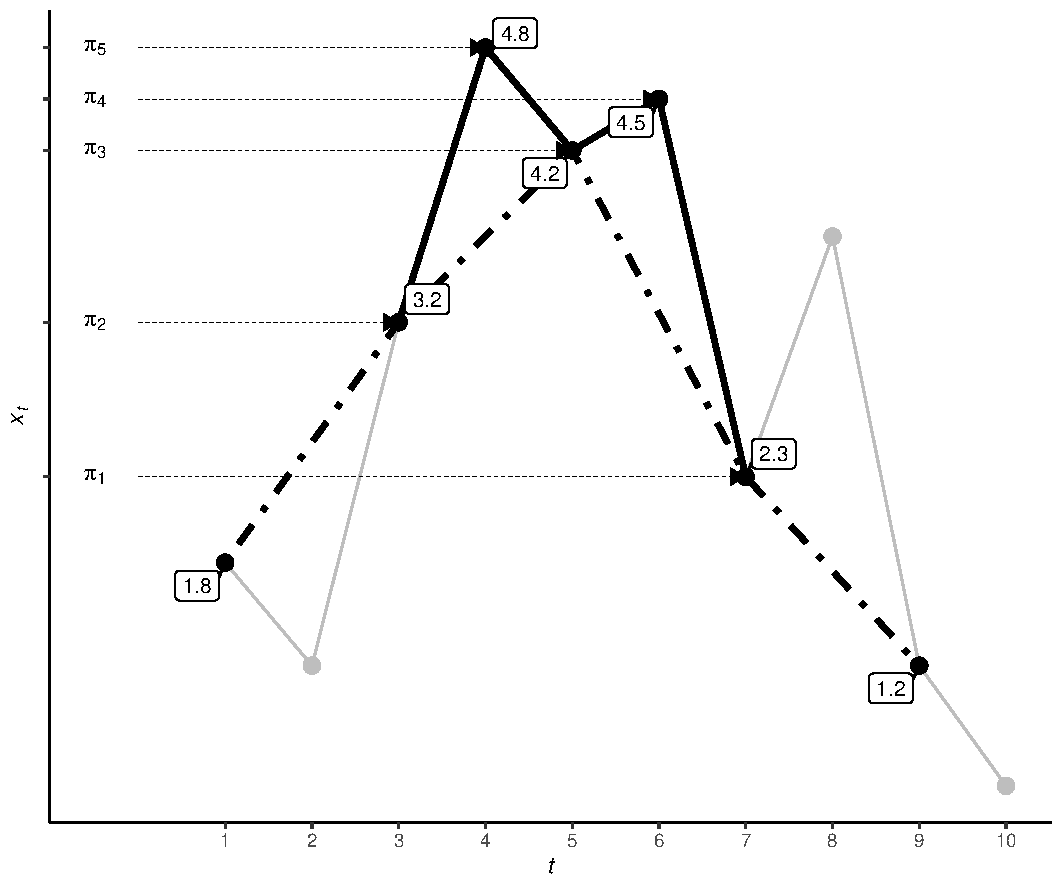
\includegraphics[width=.9\linewidth]{Figures/IntroBP.pdf}
	\caption{Illustration of the Bandt and Pompe coding\label{Fig:IntroBP}}
\end{figure}

The classic approach to calculating the probability distribution of ordinal patterns is through the frequency histogram.
Denote $\Pi$ the sequence of symbols obtained by a given series $\mathbf{X}_t^{(D,\tau)}$.
The Bandt-Pompe probability distribution is the relative frequency of symbols in the series against the $D!$ possible patterns $\{\widetilde\pi_t^D \}_{t = 1}^{D!}$:
%\todo[inline]{Não sei como, mas essa equação tem que caber na largura da página. Sugestão:
%\begin{equation}
%   p(\widetilde\pi_t^D) = \frac{\#\left \{\mathbf{X}_t^{(D,\tau)} \text{ is of type } \widetilde\pi_t^D\right \}}{T- (D-1)\tau},  
%\end{equation}
%
%where  $t\in \{1, \dots, T-(D-1)\tau\}$.
%}
%%% ETCC DONE
\begin{equation}
p(\widetilde\pi_t^D) = \frac{\#\left \{\mathbf{X}_t^{(D,\tau)} \text{ is of type } \widetilde\pi_t^D\right \}}{T- (D-1)\tau},  
\end{equation}
where  $t\in \{1, \dots, T-(D-1)\tau\}$.
These probabilities meet the conditions $p(\widetilde\pi_t^D) \ge 0$ and  $\sum_{i=1}^{D!} p(\widetilde\pi_t^D) = 1$, and are invariant before monotonic transformations of the time series values.

Recent works propose a weighting in the calculation of relative frequencies for ordinal patterns with different amplitude variances, making them contribute differently to the final value of the permutation entropy (PE) and, thus, incorporating amplitude change information~\cite{Fadlallah2013Weightedpermutation, xiao2009fine, azami2016amplitude}.
However, these methods do not consider the amplitude difference present in different time series, weighing them similarly when calculating the final value of their probabilities.
Therefore, data with different amplitudes but with similar variance dynamics are not discriminated against, losing important information about the system dynamics.

\subsection{Ordinal Pattern Transition Graph}\label{OPTG}

Alternatively, one may form an oriented graph with the transitions from $\widetilde\pi_t^D$ to $\widetilde\pi_{t+1}^D$. 
The Ordinal Pattern Transition Graph ${G} = ({V}, {E})$ 
represents the transitions between two consecutive ordinal patterns over time $t$.
The vertices are the patterns, and the edges the transitions between them:
$V = \{v_{\widetilde\pi_t^D}\}$, and 
$E = \{(v_{\widetilde\pi_t^D}, v_{\widetilde\pi_{t+1}^D}): v_{\widetilde\pi_t^D}, v_{\widetilde\pi_{t+1}^D} \in V \}$~\cite{Borges2019Transition}.

The literature reports two approaches to compute the weight of edges.
Some authors employ unweighted edges~\cite{McCullough2015lagged,Kulp2016ordinal} which represent only the existence of transitions, while others apply the frequency of transitions~\cite{Sorrentino2015periodic,Zhang2017ConstructingOP}.
The weights $\mathbb{W} = \{w_{v_{\widetilde{\pi}^D_i}, v_{\widetilde\pi^D_j}}: v_{\widetilde\pi^D_i}, v_{\widetilde\pi^D_j} \in V \}$ assigned to each edge describe the chance of transitions between the patterns $(v_{\widetilde\pi^D_i}, v_{\widetilde\pi^D_j})$
The weights are calculated as the relative frequency of each transition, i.e., as:
\begin{equation}
w_{v_{\widetilde\pi^D_i}, v_{\widetilde\pi^D_j}} = \frac{|\Pi_{\widetilde\pi^D_i,\widetilde\pi^D_j}|}{T-(D-1)\tau-1},
\end{equation}
where $|\Pi_{\widetilde\pi^D_i,\widetilde\pi^D_j}|$ is the number of transitions from pattern $\widetilde\pi^D_i$ to pattern $\widetilde\pi^D_j$, $\sum_{v_{\widetilde\pi^D_i}, v_{\widetilde\pi^D_j}}w_{v_{\widetilde\pi^D_i}, v_{\widetilde\pi^D_j}} = 1$,
and the denominator is the number of transitions between sequential patterns in the series of motifs of length $T-(D-1)\tau$.

\subsection{Weighted Ordinal Patterns Transition Graph}\label{WATG}

Our proposal for computing the probability distribution, henceforth referred to as Weighted Amplitude Transition Graph (WATG), takes into account the scattering properties of the target, leading to a good characterization of the textures.
We propose a modification of the current ordinal pattern transition graph, incorporating the absolute difference between the observations that produced the patterns.%, change the traditional distribution of the weight of the edges.

First, each $\mathcal{X}$ time series is scaled to $[0, 1]$, since we are interested in a metric able to compare datasets:
\begin{equation}
\frac{x_i - x_{\min}}{x_{\max} - x_{\min}} \longmapsto x_i,
\end{equation}
where $x_{\min}$ and $x_{\max}$ are, respectively, the minimum and maximum values of the series.
This transformation is relatively stable before contamination, e.g., if instead of $x_{\max}$ we observe $k x_{\max}$ with $k\geq 1$, the relative values are not altered. Nevertheless, other more resistant transformations as, for instance, $z$ scores, might be considered.


Each $\mathbf{X}^{(D, \tau)}_t$ vector is associated with a weight $\beta_t$ that measures the largest difference between its elements:
\begin{equation}
\beta_t = \max\{x_i - x_j\},
\end{equation}
where $x_i, x_j \in \mathbf{X}^{(D, \tau)}_t$.

We propose that the weight assigned to each edge is proportional to the amplitude difference observed in the transition:	
\begin{equation}
w_{v_{\widetilde \pi^D_i}, v_{\widetilde \pi^D_j}} =  \sum_{i : \{\mathbf{X}^{(D,\tau)}_t \mapsto \widetilde\pi^D_i\}} \sum_{j : \{\mathbf{X}^{(D,\tau)}_t \mapsto \widetilde\pi^D_j\}} |\beta_i - \beta_j| .
\end{equation}
Thus, the probability distribution taken from the weighted amplitude transition graph is given as follows:	
\begin{align}
&\left\{\begin{array}{l}
\lambda_{v_{\widetilde\pi^D_i}, v_{\widetilde\pi^D_j}} = 1, \text{ if } (v_{\widetilde\pi^D_i}, v_{\widetilde\pi^D_j}) \in {E}, \\
\lambda_{v_{\widetilde\pi^D_i}, v_{\widetilde\pi^D_j}} = 0, \text{ otherwise}.
\end{array}\right., \text{ and} \\
&p(\widetilde\pi^D_i, \widetilde\pi^D_j) = \frac{\lambda_{v_{\widetilde\pi^D_i}, v_{\widetilde\pi^D_j}} \cdot w_{v_{\widetilde\pi^D_i}, v_{\widetilde\pi^D_j}}}{\sum_{v_{\widetilde\pi^D_a}, v_{\widetilde\pi^D_b}} w_{v_{\widetilde\pi^D_a}, v_{\widetilde\pi^D_b}}}.
\end{align}

Note that the conditions $p(\widetilde\pi^D_i, \widetilde\pi^D_j) \ge 0$ and $\sum_{\widetilde\pi^D_i, \widetilde\pi^D_j} p(\widetilde\pi^D_i, \widetilde\pi^D_j) = 1$ are satisfied.

Thus, series with uniform amplitudes have edges with probability of occurrence well distributed along the graph, while those with large peaks have edges with probability of occurrence much higher than the others.

\subsection{Information-Theoretic Descriptors}\label{HC}

We chose two Information Theory descriptors: Shannon Entropy and Statistical Complexity.
Computing these quantities is the last step of the algorithm, i.e., obtaining the point in the $H \times C$ plane.

Entropy measures the disorder or unpredictability of a system characterized by a probability measure $\mathbb{P}$.

Let $\mathbb{P} = \{p_{(\widetilde\pi^D_1, \widetilde\pi^D_1)}, p_{(\widetilde\pi^D_1, \widetilde\pi^D_2)}, \dots, p_{(\widetilde\pi^D_{D!}, \widetilde\pi^D_{D!})} \} = \{p_1,\dots,p_{D!^2}\}$ be the probability function obtained from the time series weighted amplitude transition graph $\mathbb{X}$.
Its normalized Shannon entropy is given by:	
\begin{equation}
H(\mathbb{P}) = -\frac1{2\log D!}\sum_{\ell=1}^{D!^2} p_{\ell} \log p_{\ell} .
\label{eq:Entropia}
\end{equation}

The ability of the entropy to capture system properties is limited, so it is necessary to use it in conjunction with other des\-criptors to obtain a more complete analysis.
Other interesting measures are the distances between $\mathbb{P}$ and a probability measure that describes a non-informative process, typically the uniform distribution.

The Jensen-Shannon distance to the uniform distribution $\mathbb{U} = (\frac{1}{D!^2}, \dots, \frac{1}{D!^2})$ is a measure of how similar the underlying dynamics is to a non-informative process.
It is calculated as:
\begin{equation}
Q'(\mathbb{P}, \mathbb{U}) = \sum_{\ell=1}^{D!^2} \Big(p_\ell \log\frac{p_\ell}{u_\ell} +
u_\ell \log\frac{u_\ell}{p_\ell}
\Big).
\end{equation}
This quantity is also called ``disequilibrium.''
The normalized disequilibrium is $ Q=Q'/\max\{Q'\}$.

Conversely to entropy, the statistical complexity seeks to find interaction and dependence structures among the elements of a given series, being an extremely important factor in the study of dynamic systems.

The Statistical Complexity is then defined as~\cite{Lamberti2004Entropic}:
\begin{equation}
C(\mathbb{P}, \mathbb{U}) = H(\mathbb{P}) Q(\mathbb{P}, \mathbb{U}).
\end{equation}

In our analysis, each time series can then be described by a point $(H(\mathbb{P}), C(\mathbb{P}, \mathbb{U}))$.
The set of all pairs $(H(\mathbb{P}), C(\mathbb{P}, \mathbb{U}))$ for any time series described by patterns of length $D$ lies in a compact subset of $\mathbbm R^2$: the Entropy-Complexity plane.
Martin et al~\cite{martin2006generalized} obtained explicit expressions for the boundaries of this closed manifold, which depend only on the embedding dimension $D$.

Through such a tool it is possible to discover the nature of the series, determining if it corresponds to a chaotic (or other deterministic dynamics) or stochastic sequences.

\section{EXPERIMENTAL RESULTS AND ANALYSIS}\label{Results}

In this section, we describe the dataset, 
the classification process, and 
the results of the experiments.
To assess the performance of the technique here proposed, we first analyze the impact of its parameters and then compare its results in the classification with other methods.

\subsection{Image Dataset}

The proposed method was evaluated based on three quad-polarimetric L-band SAR images from the NASA Jet Propulsion Laboratory’s (JPL’s) uninhabited aerial vehicle synthetic aperture radar (UAVSAR).
We used the HH backscatter magnitudes of:
\begin{itemize}
	\item Sierra del Lacandon National Park, forest region in Guatemala (acquired on April 10, 2015)\footnote{\protect{\url{https://uavsar.jpl.nasa.gov/cgi-bin/product.pl?jobName=Lacand_30202_15043_006_150410_L090_CX_01\#dados}}};
	\item Cape Canaveral Ocean Regions (acquired on September 22, 2016);
	\item Urban area of the city of Munich, Germany (acquired on June 5, 2015)\footnote{\protect{\url{https://uavsar.jpl.nasa.gov/cgi-bin/product.pl?jobName=munich_19417_15088_002_150605_L090_CX_01\#data}}}.
\end{itemize}

We manually selected $160$ samples of size $128 \times 128$ to compose the dataset used in the experiments.
It is organized as follows:
$40$ samples from Guatemalan forest regions;
$80$ samples from the oceanic regions of Cape Canaveral, divided into two types with different contrast; and
$40$ samples of urban regions of the city of Munich.
Fig.~\ref{fig:samples} shows examples of each.

%%% ACF Isso é verdade para a simbolização de Bandt-Pompe, mas a proposta inclui uma medida das diferenças de amplitude. Precisa pensar melhor nesta afirmação
%Since the symbolization process is invariant to monotonous transformations and resistant to contamination effects, contrast changes are not capable of causing changes in the final results obtained by the descriptors.
%Thus, the different types of oceanic regions considered in this work were studied as a single more general class.

%%% ACF Não se entende
%%% ETCC Modifiquei a frase 

%In the classification, to avoid overlapping between samples and to preserve the general distribution of the classes, the training, test and validation data were determined based on a random sampling carried out in each region of analysis.
We randomly split the samples in training (\SI{85}{\percent}) and test (\SI{15}{\percent}) sets.
We used the first set to train a $k$-nearest neighbor classifier algorithm with tenfold cross-validation.
The test samples were not used in the training stage.

\subsection{Analysis of ordinal patterns methods}

Fig.~\ref{fig:timeSeries} shows examples of the ocean, forest and urban samples as sequences values, after the linearization process.
%\todo[inline]{Nessa figura 4B não seria interessante mostrar uma série temporal de cada tipo apresentado acima? Ou seja, uma de floresta, mar tipo 1 (seja lá que isso significa), mar tipo 2 (idem) e urbano?}
%%%% ETCC Figura atualizada
Data resulting from remote sensing have a peculiar feature that justifies the application in this article:
The variation in the magnitude of the targets' backscatter and, consequently, in the intensity of the image pixels, depends on the intrinsic properties of the regions under analysis.
Urban targets usually exhibit the strongest variation, followed by forests, and finally, water bodies.

By adding information related to amplitude, the proposed method is able to increase, compared to traditional methods, the granularity of information captured by ordinal patterns.
%\todo[inline]{Quais vantagens?}
%%% ETCC especifiquei que a vantagem é dada pelo aumento da granularidade de informação capturada.
Fig.~\ref{fig:plotsHC} shows the evolution of the descriptive power of these techniques.

The Bandt-Pompe symbolization was the first method based on ordinal patterns proposed in the literature.
As shown in Fig.~\ref{fig:plotsHC} left, it provides a limited separation of the textures.
Transition graphs (Fig.~\ref{fig:plotsHC} center) improve the spread of the features, but with some amount of confusion.
Our proposal, shown in Fig.~\ref{fig:plotsHC} right, produces well-separated features.

%When considering the dynamics of alternating between consecutive patterns in a sequence, the transition graphs provide more information about the reference target and, consequently, this method is able to differentiate most of these dynamics, but there are challenging situations without a clear separation between them, causing misclassifications.

%On the other hand, as discussed in the section~\ref{WATG}, the weighted graph provides greater weight for transitions between ordinal patterns that have a wide range of amplitude.
%While in the traditional graph, the weight of the edges was obtained only by the frequency of the transitions, in the proposed method the symbols that appear with the same frequency gain different importance.
In this way, we were able to obtain, for this experiment, a perfect characterization and, consequently, the high descriptive power of the regions.
%In addition, some edges may disappear if the variation in amplitude between ordinal patterns is zero.

\begin{figure*}[hbt]
	\begin{tabular}{cccc}
		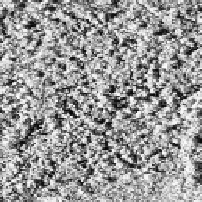
\includegraphics[width=0.22\textwidth]{Figures/guatemalaflorest.pdf} &   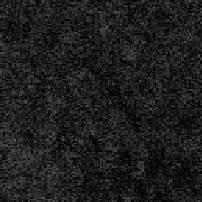
\includegraphics[width=0.22\textwidth]{Figures/Cape1.pdf} &
		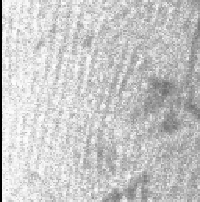
\includegraphics[width=0.22\textwidth]{Figures/Cape2.pdf} &  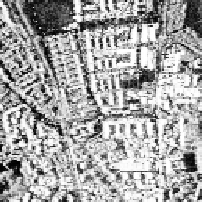
\includegraphics[width=0.22\textwidth]{Figures/munichUrban.pdf} \\
	\end{tabular}
	\caption{Types of regions analyzed: Guatemala forest, Canaveral ocean type 1,
		ocean type 2, and Munich urban area}
	\label{fig:samples}
\end{figure*}

\begin{figure*}[hbt]
	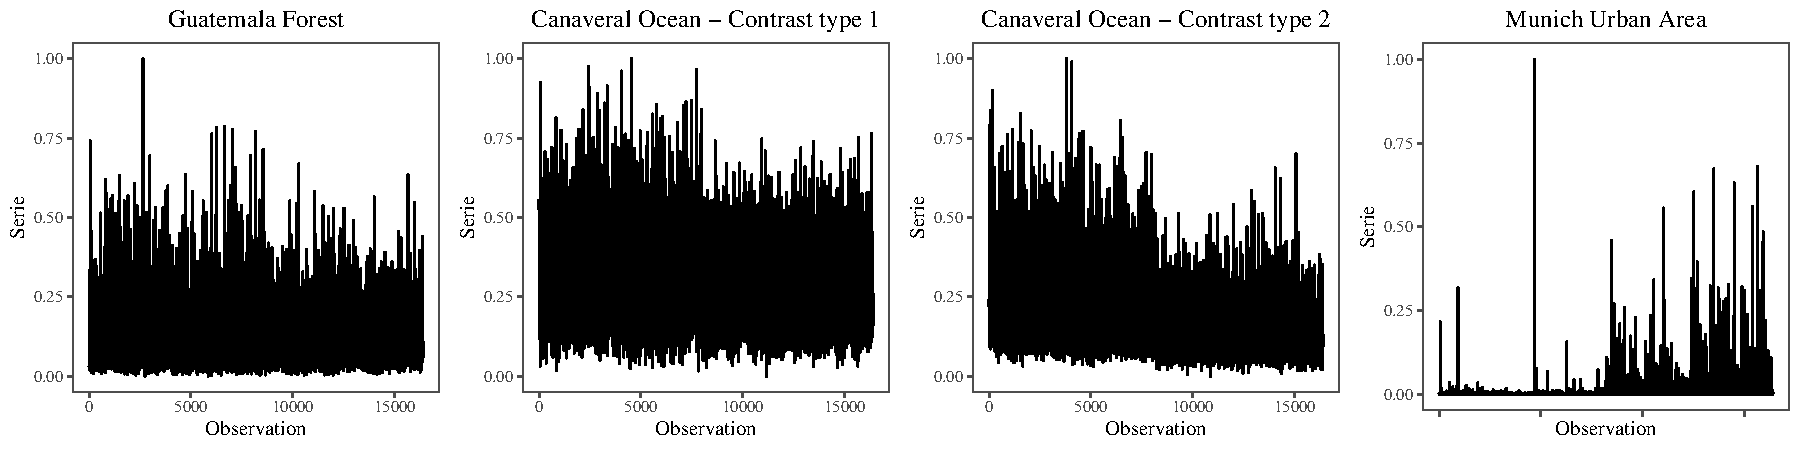
\includegraphics[width=2\columnwidth]{Figures/SAR_TS.pdf}
	\caption{Amplitude of different types of regions}
	\label{fig:timeSeries}
\end{figure*}

\begin{figure*}[hbt]
	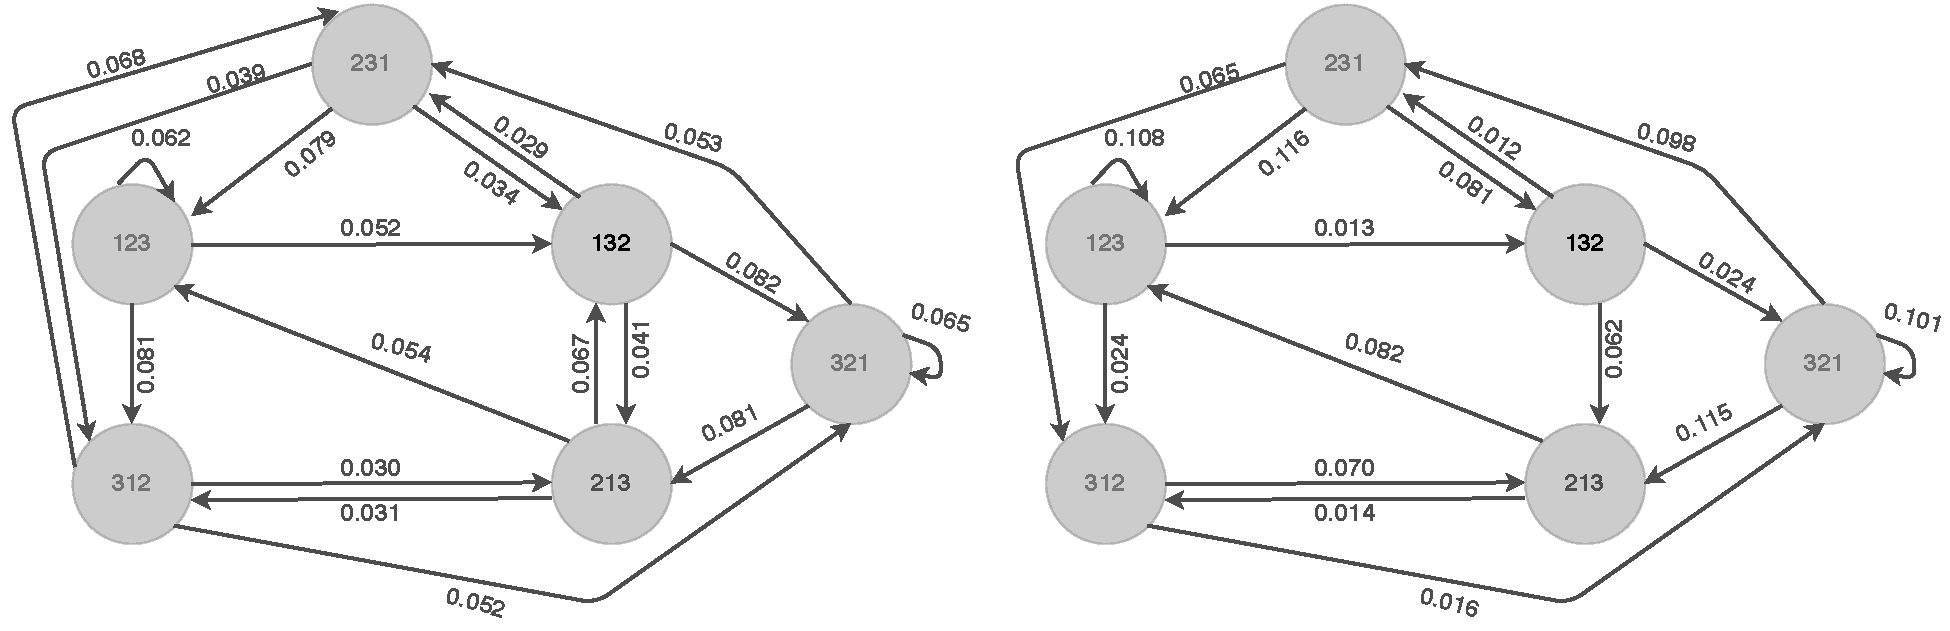
\includegraphics[width=2\columnwidth]{Figures/graphs.pdf}
	\caption{Example of the difference in weights at the edges in a sample of Munich urban regions in the transition graph and in the weighted graph of ordinal patterns
		transition to dimension 3 and delay 1}
	\label{fig:graphs}
\end{figure*}

\begin{figure*}[hbt]
	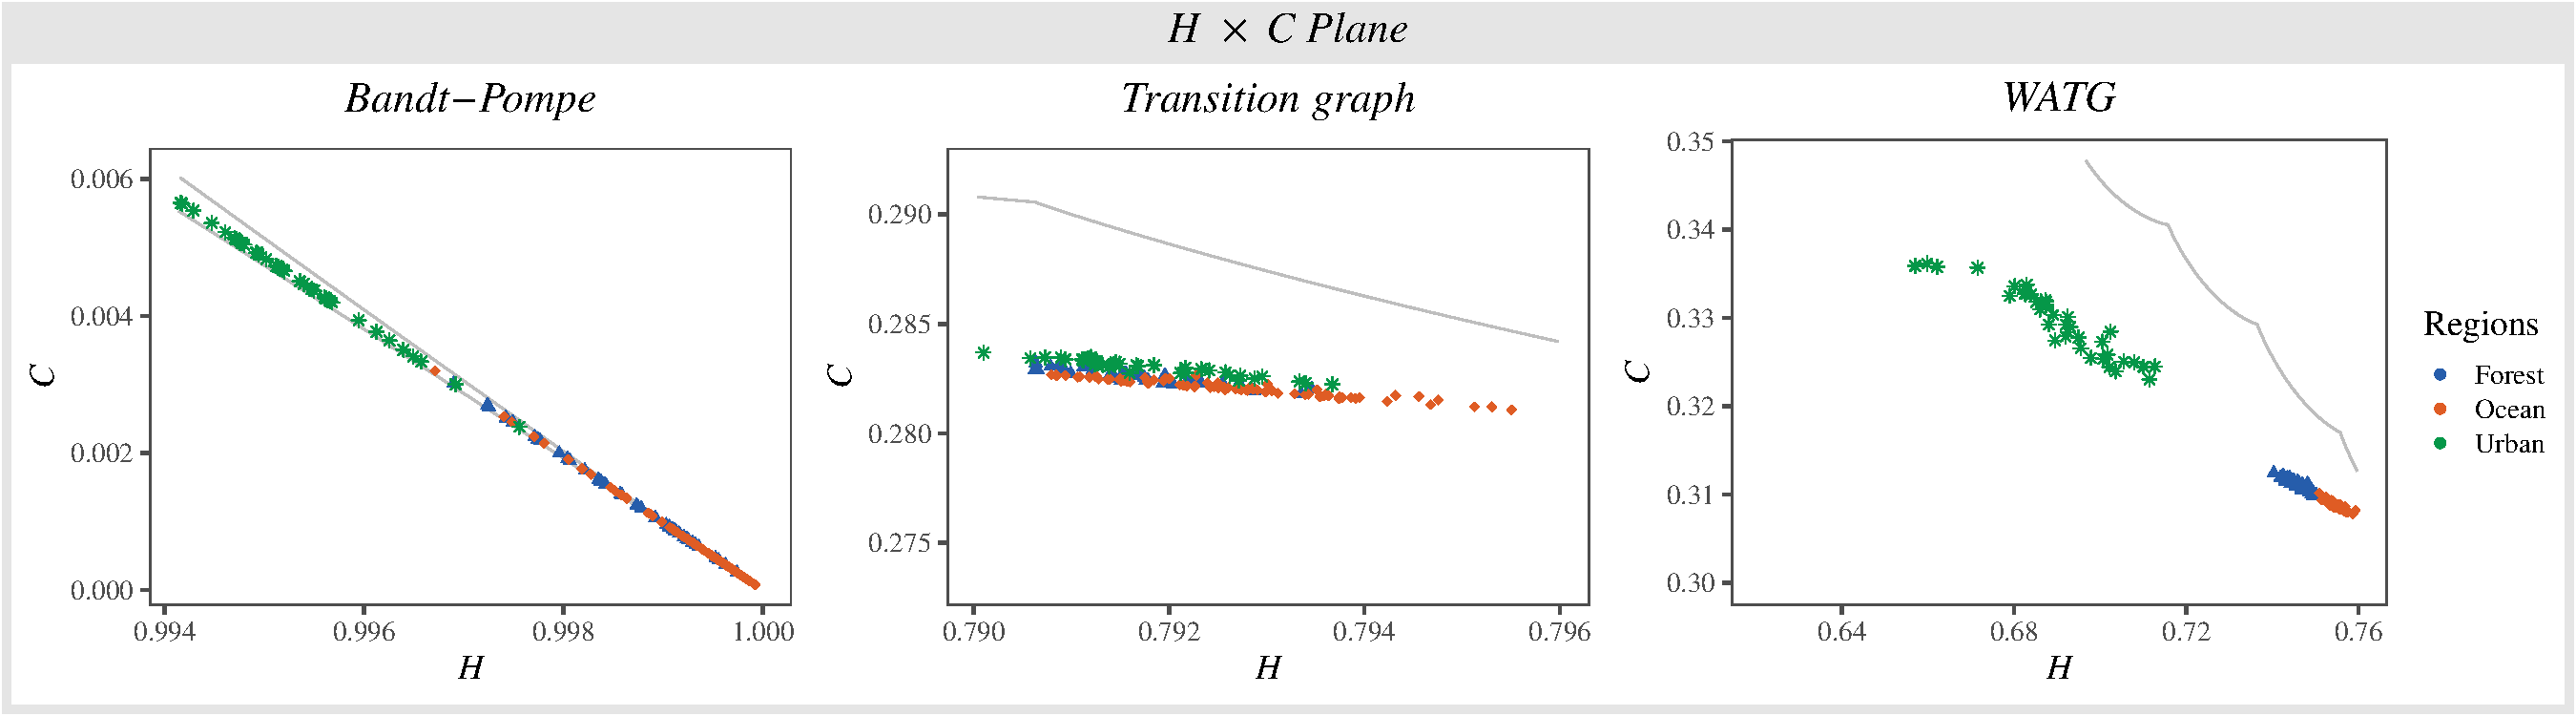
\includegraphics[width=2\columnwidth]{Figures/HCAnalysis.pdf}
	\caption{Location of Guatemala (forest), Cape Canaveral (ocean) and Munich (urban) on the HC plane for dimension 3 and delay 1.}
	\label{fig:plotsHC}
\end{figure*}

As already described in Section~\ref{WATG}, our proposal weights the edges in terms of the difference of amplitudes.
As expected, the greatest impact is observed on the transition graphs obtained from urban areas.

The urban area time series shown in Fig.~\ref{fig:timeSeries} has the largest dynamic range.
Fig.~\ref{fig:graphs} shows how this information alters the weights of the transition graph.
Notice, in particular, that 
$(v_{\widetilde \pi^3_{123}}, v_{\widetilde \pi^3_{123}})$ almost doubled, while 
$(v_{\widetilde \pi^3_{312}}, v_{\widetilde \pi^3_{231}})$ and $(v_{\widetilde \pi^3_{213}}, v_{\widetilde \pi^3_{132}})$ became negligible.

We highlight the impact of the weighting on the probability distribution in the two extreme cases observed:
\begin{itemize}
	\item If the time series presents a low amplitude variation and intensity peaks between, then the transitions of ordinal patterns that represent the latter have larger weights.
	This contributes so that the probability distribution becomes less uniform among the symbols, since it will be more concentrated in these edges.
	This will also cause a drop in the Entropy, when compared to the traditional method.
	\item In time series that show a uniform amplitude variation, the weights are well distributed between their edges, giving rise to a more random probability distribution, thus obtaining larger entropy.
\end{itemize}

%\todo[inline]{Aqui precisa destacar no grafo o que acontece, ou seja, indicar as mudanças e quais os impactos delas no problema tratado.}
%%%ETCC Adicionado nos novos parágrafos

\subsection{Experiments on sliding window selection}

In this section, we analyze the parameters of the proposed method and its impact on the classification of textures.
McCullough et al.~\cite{McCullough2015lagged} report that inadequate values may hinder important characteristics of the phenomenon under analysis.

The two parameters of the transition graph are the dimension $D$, and the delay $\tau$.
In the experiments below, we present the results in the classification using different values of these parameters.

The performance of the classification method based on ordinal patterns is sensitive to window size, the embedding dimension, and the delay.
In techniques based in Bandt-Pompe symbolization, for a fixed time series, as the size of embedding dimension decreases, more ordinal patterns are produced.
Therefore, we acquire a greater granularity of information about the dynamics of the system and, consequently, we capture more spatial dependencies between the elements.
%\todo[inline]{acho que essa afirmação é bem forte, não teria que argumentar melhor? Para mim não ficou claro o fato de que mais padrões aparecem quando tau é menor. Tem referências para isso?}
%%%ETCC reescrevi a sentença, acredito que agora esteja melhor

We used the ROC curve shown in Fig.~\ref{fig:ROC} for different values of $D \in \{3, 4, 5, 6 \} $ and $\tau \in \{1, 2, 3, 4, 5 \}$ to select the best configuration.

\begin{figure}[hbt]
	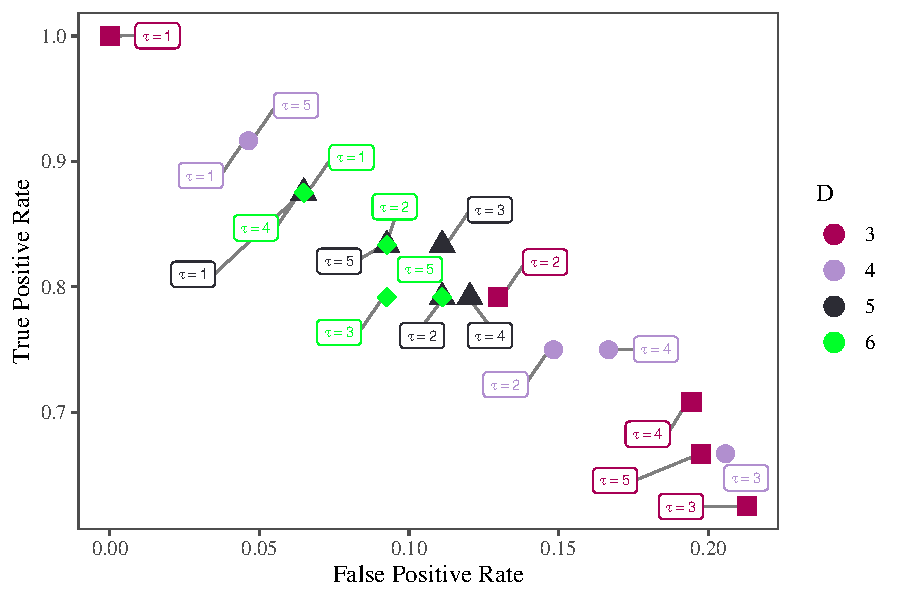
\includegraphics[width=\columnwidth]{Figures/ROC.pdf}
	\caption{Evaluation of the sliding window parameters}
	\label{fig:ROC}
\end{figure} 

As we can see in Fig.~\ref{fig:ROC}, the configuration that extracted most information from the time series and, thus, that presented the best results in the experiments, is $D = 3$ and $\tau = 1$.
%\todo[inline]{aqui também eu não entendi porque D=3 e tau=1 garante que aumenta o nível de informação extraída. Tem que ter um certo cuidado com essas afirmações muito fortes. Tem referências para isso? Como podemos concluir isso apenas por essa análise? Talvez isso valha para esse experimento, se for isso, tem que ser melhor descrito}
%%% ETCC a frase foi reescrita, realmente acabou passando outra informação sobre o que eu queria repassar
The technique, thus, shows its best performance choosing the parameters with the lowest computational cost.

Figure~\ref{fig:Regions} shows the points in the $H\times C$ produced by the same samples with all the parameters mentioned above.
The spatial distribution of the points changes with the parameters,
and certain configurations promote better separation.
%\todo[inline]{Não consegui ver novos grupos de padrões aparecendo. A figura não mostra os padrões, apenas os valores de HxC}
%%%ETCC frase reescrita

We obtain the lowest Entropy and the largest Statistical Complexity
in urban areas 	with $ D = 3 $ and $ \tau = 1 $.
%When we apply small values of delay and dimension in WATG to data from the urban region (for example, as with $ D = 3 $ and $ \tau = 1 $), we obtain the lowest entropy values and the highest statistical complexities values of the dataset, which is justified by the peak values present in their sequences, as seen in Fig~\ref{fig:example}b.
%\todo[inline]{isso também não fica claro nessa figura, talvez fique na série temporal}
%%%ETCC frase reescrita
The Statistical Complexity discriminates best ocean and forest regions.
%have as their main discriminating descriptor the statistical complexity that portrays the degree of temporal dependence structure between the symbols and consequently between the pixel intensity values.

Fig.~\ref{fig:Regions} shows the WATG points dimension values $D$ and delays $\tau$.
%Since such values inform us of intrinsic characteristics of the dynamics of the series in their specific domains, inadequate values may hide this kind of knowledge about the data, and this analysis step is crucial.
%
This figure shows that discrimination ability decreases with increasing $\tau$.
Larger values of delay dilute the spatial dependence, as neighboring points in the sample tend to be more distant in the image.
For this reason, we will use $\tau=1$.
%\todo[inline]{Isso não estaria relacionado ao fato de que valores maiores de tau faria com que se perdesse a estrutura de dependência espacial pois os pontos vizinhos na amostra tendem a ficar mais distantes na imagem?}
%%%ETCC Realmente. Frase alterada

Considering $\tau=1$ (first column of Fig.~\ref{fig:Regions}), 
we also notice that $D=3$ produces the best separation among classes.
Increasing $D$ also increases the Statistical Complexity; this is noticeable for the Forest class.
The other effect of considering larger values of $D$ is an increased Entropy of Ocean and, with it, an undesirable overlap with Urban samples.

%As WATG captures amplitude differences between different time series, when the values of the $\tau$ scale increase, well-distributed weight plots are formed, thus obtaining increasing entropy values.
%On the other hand, as we increase $D$, the granularity of the information increases, capturing more spatial dependence structures in the data and, consequently, acquiring greater statistical complexity.
%There is a relationship between the dimension variable of ordinal patterns and the discrimination between the analyzed regions that presents its best result for $D = 3$.
%On the other hand, when we have $D = 6$, textures acquire a lower entropy value and become harder to distinguish.
%\todo[inline]{Acho que é bom usar transparência nos pontos para a gente perceber que tem sobreposição de classes em alguns casos em que D=3 de Tau=1 é a configuração que separa melhor as classes}
%%%ETCC transparência foi adicionada nos pontos

\begin{sidewaysfigure*}
	\centering
	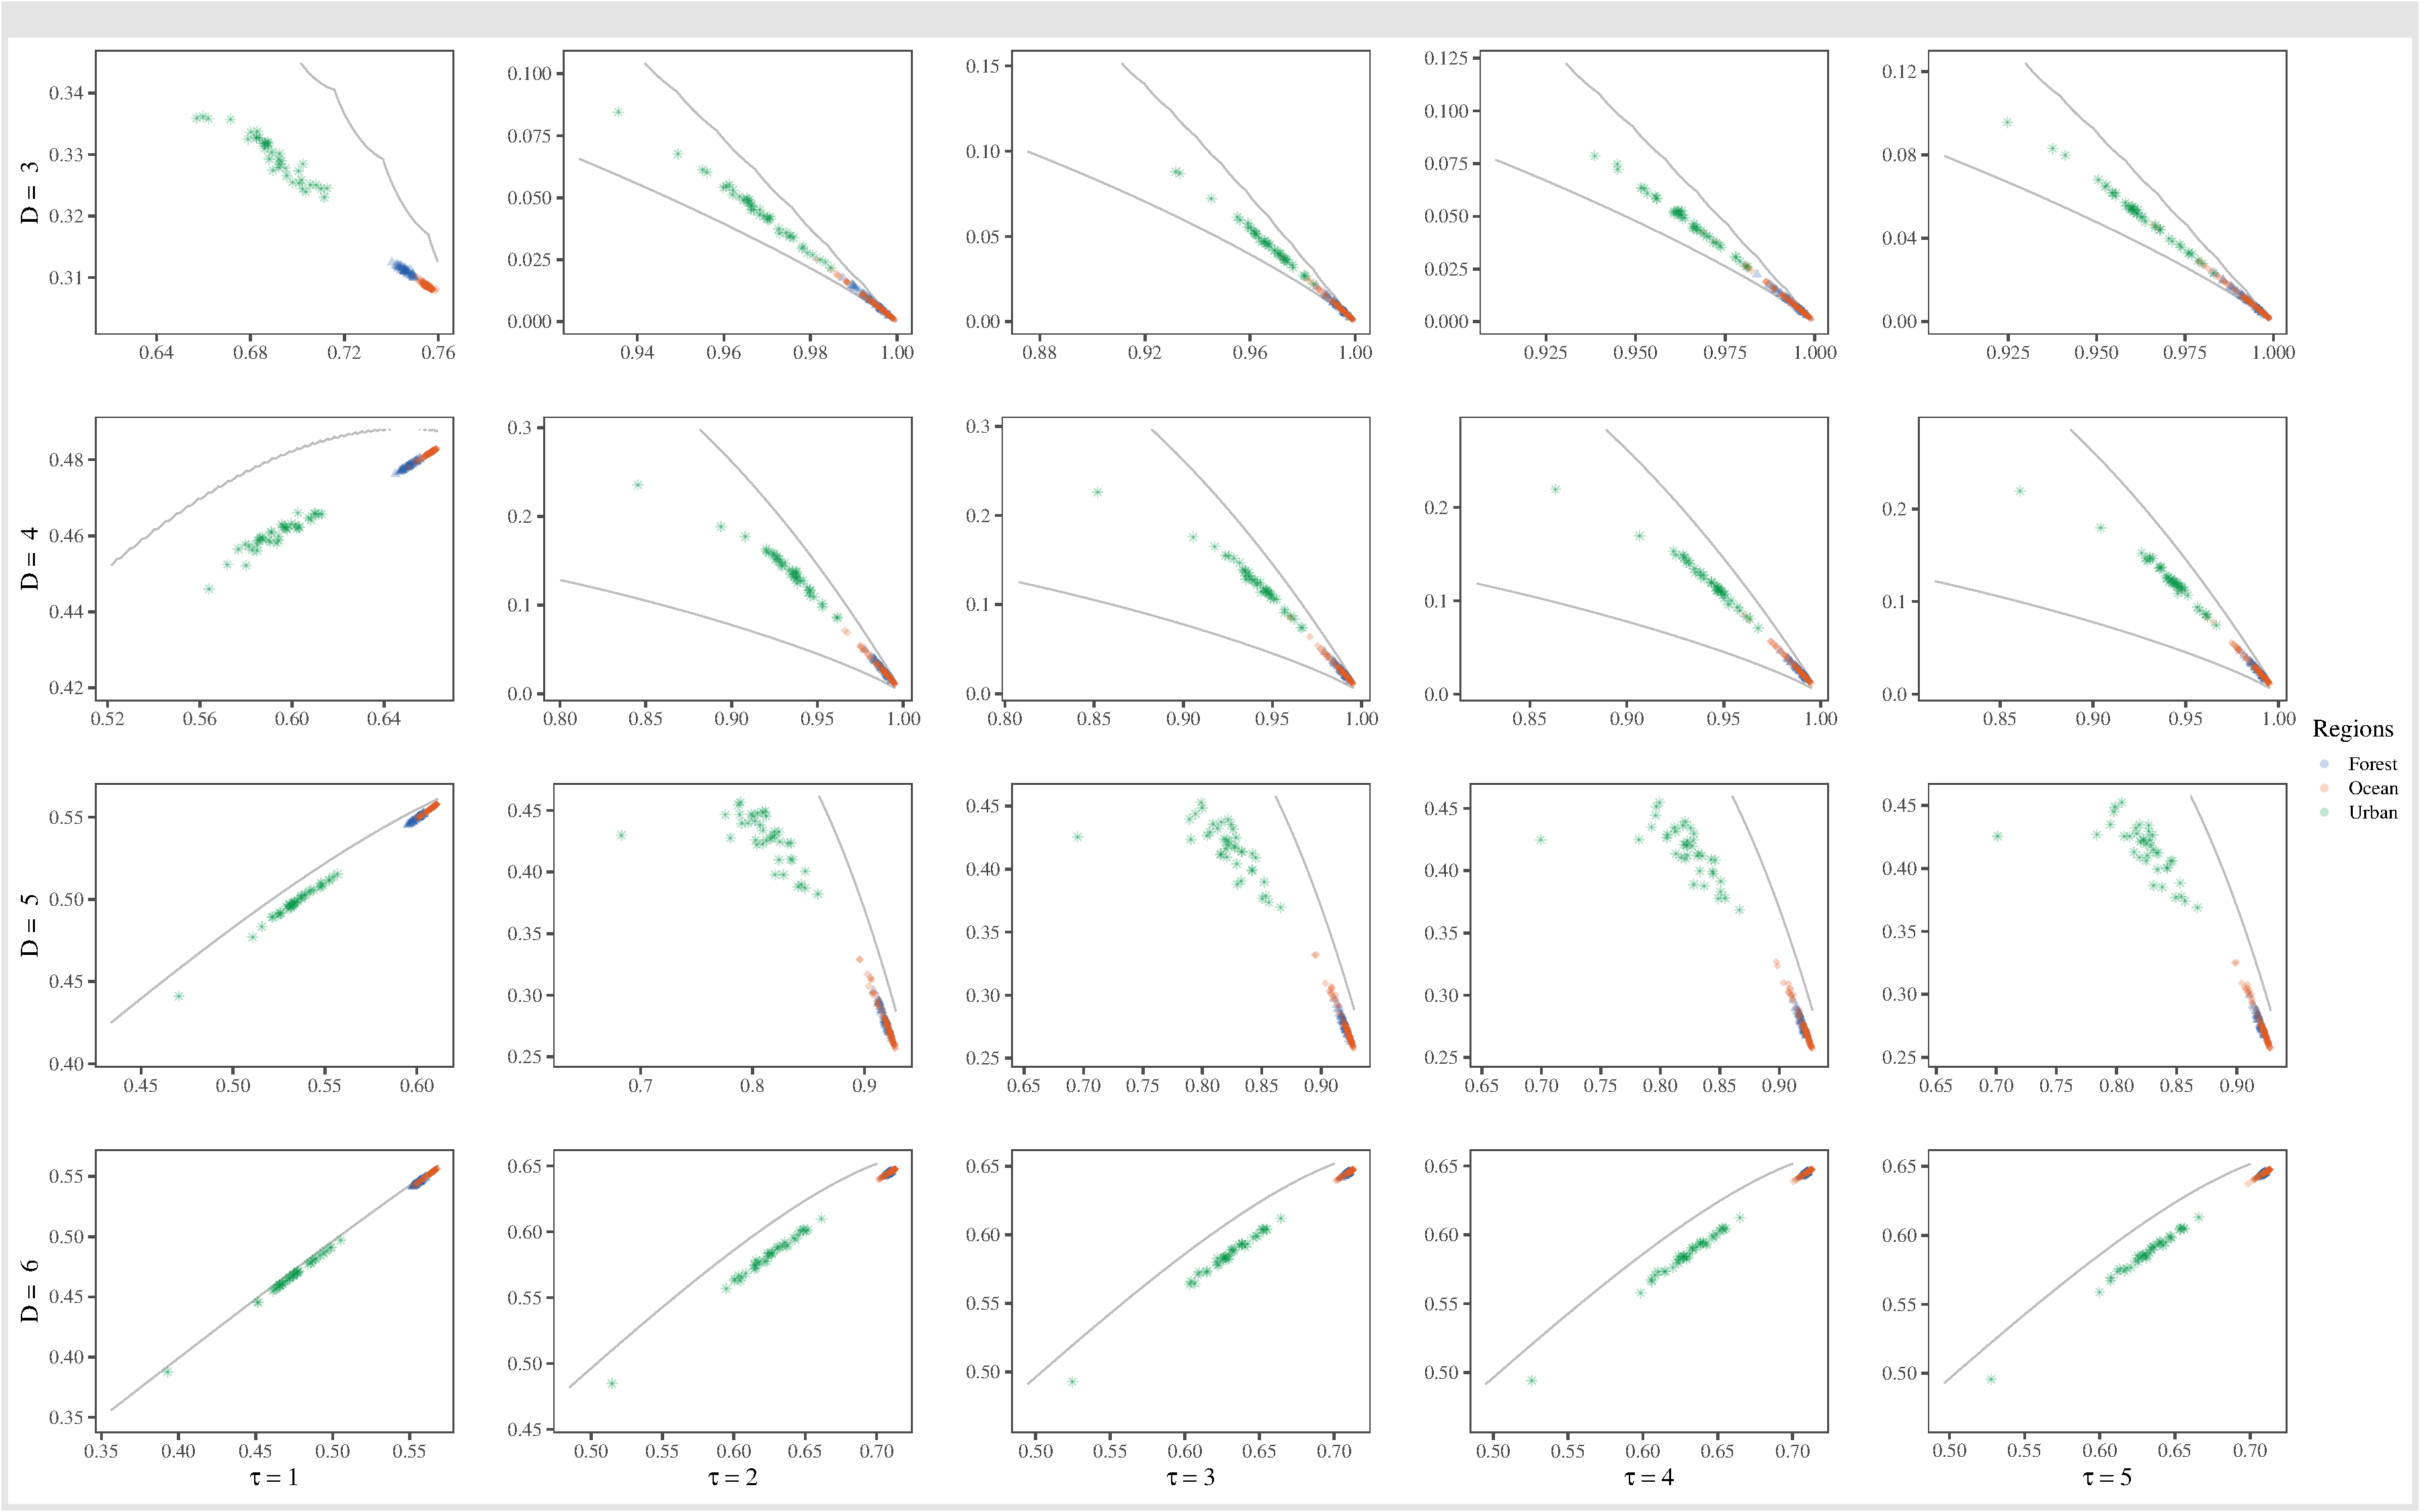
\includegraphics[width=1\textwidth]{Figures/WATGHC.pdf}
	\caption{Characterization resulting in HC Plane from the application of the Hilbert-Peano curve in WATG on textures of different regions: Guatemala (forest), Cape Canaveral (ocean) and Munich (urban).}
	\label{fig:Regions}
\end{sidewaysfigure*}

\subsection{Quantitative Evaluation}

%Several experiments were carried out to validate the features extracted from the information theory descriptors in the characterization and classification of regions.
We present a comparison between our proposal and other methods for characterization and texture classification.
We use the following eight methods: 
Gray-level co-occurrence matrices~\cite{kourgli2012texture}, 
Gabor filters~\cite{weldon1996efficient},  
Bandt-Pompe probability distribution~\cite{Bandt2002Permutation}, 
Weighted- permutation entropy~\cite{Fadlallah2013Weightedpermutation},
Fine-grained permutation entropy~\cite{xiao2009fine}, 
Amplitude-aware permutation entropy~\cite{azami2016amplitude} and 
Ordinal patterns transition graphs~\cite{Borges2019Transition}.
As applied in~\cite{guan2019covariance}, 
we computed four statistics from co-occurrence matrices: contrast, correlation, energy, and homogeneity.
Likewise, we implemented the Gabor filters in five scales and eight orientations; using the Energy, we obtained an $80$-dimensional feature vector for each patch.
%\todo[inline]{Referências para os métodos são super bem-vindas aqui}
%%% ETCC Todos os métodos estão com referências para os seus respectivos trabalhos e adicionei o paper utilizado como referência na implementação do baseline proposto.
Table~\ref{tab:result1} summarizes the number of features each method produces.


We used the $k$-nearest neighbors algorithm for classification with Euclidean distance, selecting the value of $k$ with the automatic grid search method of the Caret R package~\cite{kuhn2008building}.
In the following, we used $k = 20$.
For validation, we used $10$-fold cross-validation.
More details about the classifier and the sampling can be seen in~\cite{mitchell1997machine}.

Table~\ref{tab:result1} presents the results of classifying the $160$ samples.
We assess the effectiveness of each approach using the following metrics: recall or True Positive Rate (TPR), precision or Positive Predictive Value (PPV), Overall Accuracy (OA), and F1-score.

\begin{table*}[hbt]
	\centering
	\caption{Experimental results using $k$-NN}
	\label{tab:result1}
	\begin{tabular}{l*9{r}}
		\toprule
		Method      & \multirow{2}{*}{\# features}         &       & TPR   &       &       & PPV    &       & \multirow{2}{*}{OA}  & \multirow{2}{*}{F1-Score} \\ \cmidrule(lr){3-5} \cmidrule(lr){6-8}
		&   & Urban & Forest & Ocean & Urban & Forest & Ocean & &  \\ \midrule
		Bandt-Pompe   & 2 & 0.833 &  0.666  & 0.833 & 1.000 & 0.571  & 0.833 & 0.792 &  0.615  \\ 
		WPE   & 2 & 0.833 &  0.666  & 0.666 & 0.833 & 0.500  & 0.800 & 0.708 &  0.571  \\ 
		FGPE ($\alpha$ = 1)  & 2 & 1.000 &  0.833  & 0.833 & 1.000 & 0.714  & 0.909 & 0.875 &  0.769  \\ 
		FGPE ($\alpha$ = 0.5)   & 2 & 1.000 &  0.833  & 1.000 & 1.000 & 1.000  & 0.923 & 0.958 &  0.909  \\ 
		AAPE (A = 1)   & 2 & 1.000 &  0.500  & 0.750  & 1.000 & 0.500  & 0.750  & 0.750 &  0.500  \\ 
		AAPE (A = 0.5)   & 2 & 1.000 &  0.333  & 0.833 & 1.000 & 0.500  & 0.714 & 0.750 &  0.400  \\ 
		Transition Graph & 2  & 1.000 & 0.666  & 0.916 & 0.857 & 1.000  & 0.846 & 0.875 & 0.800 \\
		WATG        & 2  & 1.000 & 1.000  & 1.000 & 1.000 & 1.000  & 1.000 & 1.000 & 1.000 \\ 
		Gabor           & 80  & 1.000 & 1.000  & 1.000 & 1.000 & 1.000  & 1.000 & 1.000 & 1.000\\
		GLCM            & 4   & 1.000 & 0.833  & 1.000 & 1.000 & 1.000  & 0.923 & 0.666 & 0.800\\
		\bottomrule
	\end{tabular}
\end{table*}

GLCM produced the worst overall accuracy results: $\text{OA}=\SI{66.6}{\percent}$ and $\text{F1-score}=\SI{80.0}{\percent}$.
%
On the other hand, AAPE (with $\alpha = 0.5$) produced the worst F1-score results:
$\text{OA}=\SI{75.0}{\percent}$ and $\text{F1-score}=\SI{40.0}{\percent}$.
%
Transitions graphs improve these classification results, leading to  $\text{OA}=\SI{83.3}{\percent}$ and $\text{F1-score}=\SI{60.0}{\percent}$.
%
Although better ($\text{OA}=\SI{95.8}{\percent}$ and $\text{F1-score}=\SI{90.9}{\percent}$), FGPE (with $A = 1$) is not able to have high descriptive power in the proposed dataset.
%
Both Gabor filters and the proposed method have the highest success rate $\text{OA}=\SI{100}{\percent}$ and $\text{F1-score}=\SI{100}{\percent}$.
Thus, WATG attains this performance with $2$ features instead of the $80$ employed by Gabor filters.
This reduction implies less computational power requirement and avoids the curse of dimensionality~\cite{TheCursesofDimensionality2018}.

\section{CONCLUSION}\label{Conclusion}

We presented and assessed a new method of analysis and classification of SAR image textures.
This method consists of three steps: 
(1)~linearization, 
(2)~computing the Weighted Ordinal Pattern Transition Graph, and 
(3)~obtaining Information Theory descriptors.

The method consists in finding a probability distribution function of ordinal patterns which is sensitive to amplitude information.
% and that, due to the backscattering properties of the SAR image sensors, classifies different regions of analysis.
We then applied the $k$-NN algorithm to classify the descriptors.

Experiments using patches from UAVSAR images showed that the proposal performs better than GLCM, Bandt-Pompe, Transition Graphs, and other techniques of amplitude information analysis in ordinal patterns and that it provides the same quality of results obtained with Gabor filters.
However, while Gabor filters employ $80$ features, our proposal requires only two.

As a result, in addition to perfectly separating urban areas from the others analyzed by entropy values, we are still able to differentiate oceanic and forest areas through their different values of statistical complexity, which informs us of the degree of spatial dependence between their elements.

%%% ACF Novamente, Bandt & Pompe é invariante, mas como usamos o valor absoluto das diferenças, isso deve ser melhor pensado
%%% ETCC concordo que não podemos garantir essa conclusão
%The proposed method is also invariant to monotonous transformations and resistant to the effects of contamination, even changes, in contrast, do not cause changes in the descriptors of the images.

%In the future, we hope to continue to refine the extraction of texture features, proposing an extension of the algorithm for the segmentation of regions and investigate the effects of their use in other applications e.g., erosion monitoring and urban activities.


\section{SOURCE CODE AVAILABILITY} 

%%% ACF Precisa gerar uma página HTML
%%% ETCC Providenciarei
The text, source code, and data used in this study are available at the \textit{SAR-WATG} repository \url{https://github.com/EduardaChagas/SAR-WATG}.

\bibliographystyle{IEEEtran}
\bibliography{../../../Common/sar.bib}

\section*{ACKNOWLEDGEMENTS}\label{ACKNOWLEDGEMENTS}

This work was partially funded by the Coordination for the Improvement of Higher Education Personnel (CAPES) and National Council for Scientific and Technological Development (CNPq).

\end{document}  
